\documentclass[12pt,a4paper]{article}

\usepackage[utf8]{inputenc}
\usepackage[T2A]{fontenc}
\usepackage[ukrainian]{babel}

\usepackage{geometry}
\geometry{left=2cm,right=2cm,top=2cm,bottom=2cm}

\usepackage{graphicx}
\usepackage{array,multirow}
\usepackage{booktabs}
\usepackage{caption}
\renewcommand{\thetable}{№\arabic{table}}
\captionsetup[table]{name=Таблиця}

\usepackage{amsmath}
\usepackage{pdflscape}
\usepackage{xcolor}

\usepackage{minted}

\usemintedstyle{friendly} % або monokai / vs / colorful
\setminted{linenos, breaklines, frame=single, fontsize=\small}

\usepackage{hyperref}

\begin{document}

    \begin{titlepage}

        % Картинка шапки (по центру, з відступом від верху)
        \begin{center}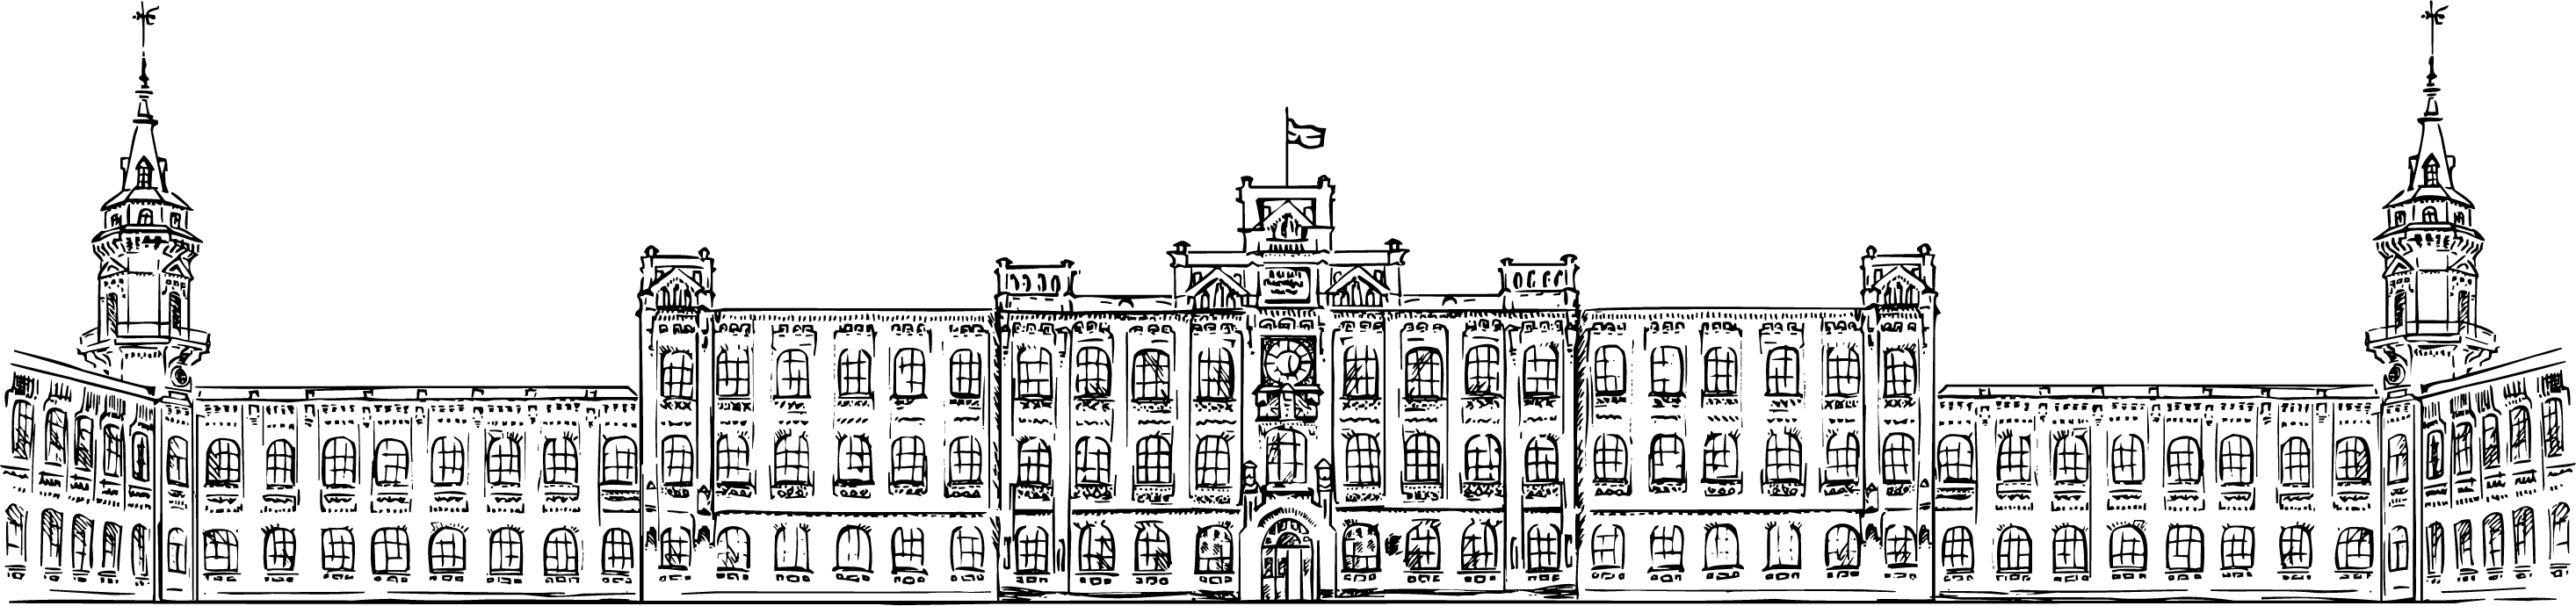
\includegraphics[width=0.7\textwidth]{../../../../TITLES/letterhead.png}\end{center}

        \begin{center}
            \large Національний технічний університет України\\
            «Київський політехнічний інститут імені Ігоря Сікорського»\\[1em]
            Факультет інформатики та обчислювальної техніки\\
            Кафедра обчислювальної техніки
        \end{center}

        \vfill

        \begin{center}
            \textbf{\LARGE Вступ до операційної системи Linux. Курсова робота}\\[2.5em]
            \textbf{\Large Лабораторна робота №2}\\
            «Введення в GIT»
        \end{center}

        \vfill

        \begin{flushright}
            Виконав: студент 2 курсу ФІОТ, гр. ІО-41\\
            \textit{Давидчук А.~М.}\\[1em]
            Перевірив: \textit{Нікольський С.~С.}
        \end{flushright}

        \vfill

        \begin{center}Київ --- 2025\end{center}

    \end{titlepage}

    % Основний документ:

    \setlength{\parindent}{0em}

    \textbf{\underline{Тема:}} «Введення в GIT».
    
    \vspace{1em}

    \begin{center} \textbf{\Large Практична частина} \end{center}

    Клонуємо репозиторій та переходимо до робочої папки calculator:
    \begin{minted}{bash}
PS C:\Users\artem\OneDrive\Desktop\lab2> git clone https://github.com/SergiiPiatakov/calculator.git
Cloning into 'calculator'...
remote: Enumerating objects: 24, done.
remote: Counting objects: 100% (14/14), done.
remote: Compressing objects: 100% (10/10), done.
remote: Total 24 (delta 5), reused 4 (delta 4), pack-reused 10 (from 1)
Receiving objects: 100% (24/24), done.
Resolving deltas: 100% (5/5), done.
PS C:\Users\artem\OneDrive\Desktop\lab2> cd .\calculator\
    \end{minted}

    Перевірка:
    \begin{minted}{bash}
PS C:\Users\artem\OneDrive\Desktop\lab2\calculator> git log --oneline
4ad40a3 (HEAD -> master, origin/master, origin/HEAD) fix truncation error
cbcb06d formatting: use tabs instead of spaces
669f632 improve calculation accuracy
976f691 add a subtraction operation
f03784b add header guard
9972170 basic implementation
75c0e7c Initial commit
    \end{minted}

    Міняю місцями коміти "\texttt{fix truncation error (4ad40a3)}" та "\texttt{formatting: use tabs}
    
    \texttt{instead of spaces (cbcb06d)}" \, за допомогою \texttt{git rebase -i HEAD~n}:
    \begin{minted}{bash}
PS C:\Users\artem\OneDrive\Desktop\lab2\calculator> git rebase -i HEAD~2
hint: Waiting for your editor to close the file...
    \end{minted}

    В редакторі:
    \begin{minted}{bash}
pick cbcb06d # formatting: use tabs instead of spaces
pick 4ad40a3 # fix truncation error

# Rebase 669f632..4ad40a3 onto 669f632 (2 commands)
#
# Commands:
...
    \end{minted}

    Міняю місцями "\texttt{pick cbcb06d ...}" та "\texttt{pick 4ad40a3 ...}", зберігаю та закриваю вікно і отримую конфлікт:

    \begin{minted}{bash}
Auto-merging calculator.cpp
CONFLICT (content): Merge conflict in calculator.cpp
error: could not apply 4ad40a3... fix truncation error
hint: Resolve all conflicts manually, mark them as resolved with
hint: "git add/rm <conflicted_files>", then run "git rebase --continue".
hint: You can instead skip this commit: run "git rebase --skip".
hint: To abort and get back to the state before "git rebase", run "git rebase --abort".
hint: Disable this message with "git config set advice.mergeConflict false"
Could not apply 4ad40a3... # fix truncation error
    \end{minted}

    Вирішую в редакторі конфлікти у обох файлів у редакторі, додаю їх до \texttt{staging area}, продовжую процес \texttt{rebase} оновлюючи текст повідомлення
    комітів, додавши від себе уточнення \texttt{rearranged} і \texttt{Edited-(rearranged)-by: Davydchuk Artem <marshal.dyachenko@gmail}

    \texttt{.com>}:
    \begin{minted}{bash}
hint: Resolve all conflicts manually, mark them as resolved with
hint: "git add/rm <conflicted_files>", then run "git rebase --continue".
hint: You can instead skip this commit: run "git rebase --skip".
hint: To abort and get back to the state before "git rebase", run "git rebase --abort".
hint: Disable this message with "git config set advice.mergeConflict false"
Could not apply 4ad40a3... # fix truncation error
PS C:\Users\artem\OneDrive\Desktop\lab2\calculator> git add .\calculator.cpp
PS C:\Users\artem\OneDrive\Desktop\lab2\calculator> git rebase --continue 
[detached HEAD 8149318] fix truncation error [rearranged]
 Author: Sergii Piatakov <sergii.piatakov@globallogic.com>
 1 file changed, 1 insertion(+), 1 deletion(-)
Auto-merging calculator.cpp
CONFLICT (content): Merge conflict in calculator.cpp
error: could not apply cbcb06d... formatting: use tabs instead of spaces
hint: Resolve all conflicts manually, mark them as resolved with
hint: "git add/rm <conflicted_files>", then run "git rebase --continue".
hint: You can instead skip this commit: run "git rebase --skip".
hint: To abort and get back to the state before "git rebase", run "git rebase --abort".
hint: Disable this message with "git config set advice.mergeConflict false"
Could not apply cbcb06d... # formatting: use tabs instead of spaces
PS C:\Users\artem\OneDrive\Desktop\lab2\calculator> git add .\calculator.cpp
PS C:\Users\artem\OneDrive\Desktop\lab2\calculator> git rebase --continue 
[detached HEAD 27bda0c] formatting: use tabs instead of spaces [rearranged]
 Author: Sergii Piatakov <sergii.piatakov@globallogic.com>
 2 files changed, 5 insertions(+), 5 deletions(-)
Successfully rebased and updated refs/heads/master.
    \end{minted}

    Тепер дивимось результат:
    \begin{minted}{bash}
PS C:\Users\artem\OneDrive\Desktop\lab2\calculator> git log -3
commit 27bda0c6f5e3f4a474c1a04ea8d37fce1084f1b4 (HEAD -> master)
Author: Sergii Piatakov <sergii.piatakov@globallogic.com>
Date:   Thu Nov 15 15:26:35 2018 +0200

    formatting: use tabs instead of spaces [rearranged]

    Signed-off-by: Sergii Piatakov <sergii.piatakov@globallogic.com>
    Edited-(rearranged)-by: Davydchuk Artem <marshal.dyachenko@gmail.com>

commit 814931806e4b33dd2f09ef9894bed5f710133c2a
Author: Sergii Piatakov <sergii.piatakov@globallogic.com>
Date:   Thu Nov 15 15:28:04 2018 +0200

    fix truncation error [rearranged]

    To convert float to integer the truncation is performed, but the
    rounding is expected.

    Test: Add (4.9, 4.9) should return 10.
    Signed-off-by: Sergii Piatakov <sergii.piatakov@globallogic.com>
    Edited-(rearranged)-by: Davydchuk Artem <marshal.dyachenko@gmail.com>

commit 669f6321a41da2337d975872e9294b8b91139010
Author: Sergii Piatakov <sergii.piatakov@globallogic.com>
Date:   Thu Nov 15 15:21:34 2018 +0200

    improve calculation accuracy

    Allow using float point arguments to avoid truncation.

    Test: Add (4.9, 4.9) should return 10.
    Signed-off-by: Sergii Piatakov <sergii.piatakov@globallogic.com>
    \end{minted}

    Створюємо два патчі в окремій папці \texttt{patches\_step1}, використовуючи "\texttt{git format-patch} ":
    \begin{minted}{bash}
PS C:\Users\artem\OneDrive\Desktop\lab2\calculator> mkdir patches_step1


    Directory: C:\Users\artem\OneDrive\Desktop\lab2\calculator


Mode                 LastWriteTime         Length Name
----                 -------------         ------ ----
d-----        01.10.2025     14:50                patches_step1


PS C:\Users\artem\OneDrive\Desktop\lab2\calculator> git format-patch -2 -o patches_step1
patches_step1/0001-fix-truncation-error-rearranged.patch
patches_step1/0002-formatting-use-tabs-instead-of-spaces-rearranged.patch
    \end{minted}

    Тепер поєднаю "\texttt{improve calculation accuracy}"\,та "\texttt{fix truncation error}"\,в один коміт, використовуючи \texttt{git rebase -i}:

    \begin{minted}{bash}
PS C:\Users\artem\OneDrive\Desktop\lab2\calculator> git rebase -i HEAD~3
hint: Waiting for your editor to close the file...
    \end{minted}

    В редакторі маю таке:
    \begin{minted}{bash}
pick 669f632 # improve calculation accuracy
pick 8149318 # fix truncation error [rearranged]
pick 27bda0c # formatting: use tabs instead of spaces [rearranged]

# Rebase 976f691..27bda0c onto 976f691 (3 commands)
#
# Commands
...
    \end{minted}

    І тут я коміт "\texttt{fix truncation error [rearranged]}" я позначу як \texttt{squash} щоб він злився у попередній
    "\texttt{improve calculation accuracy}":
    \begin{minted}{bash}
pick 669f632 # improve calculation accuracy
squash 7e1603b # fix truncation error [rearranged]
pick fcf6e73 # formatting: use tabs instead of spaces [rearranged]

# Rebase 976f691..fcf6e73 onto 976f691 (3 commands)
#
# Commands:
...
    \end{minted}

    Зберігаю, закриваю та пишу повідомлення до коміту "\texttt{improve calculation accuracy and fix truncation error}"\,зі своєю відміткою авторства
\begin{minted}{bash}
PS C:\Users\artem\OneDrive\Desktop\lab2\calculator> git log --oneline -3
3ec3990 (HEAD -> master) formatting: use tabs instead of spaces [rearranged]
56d74f3 improve calculation accuracy and fix truncation error
976f691 add a subtraction operation
    \end{minted}

    Тепер видаляю верхній коміт \texttt{"formatting: use tabs instead of spaces [rearranged]"} шляхом \texttt{git rebase -i}:

    \begin{minted}{bash}
PS C:\Users\artem\OneDrive\Desktop\lab2\calculator> git rebase -i HEAD~1
    \end{minted}

    І отримую таке в редакторі, де я зміню стан коміта \texttt{pick} на \texttt{drop} щоб видалити його зі історії
    \begin{minted}{bash}
pick 3ec3990 # formatting: use tabs instead of spaces [rearranged]

# Rebase 56d74f3..3ec3990 onto 56d74f3 (1 command)
#
# Commands:
...
    \end{minted}

    Потім зберігаю та закриваю вікно редагування та перевіряю:
    \begin{minted}{bash}
PS C:\Users\artem\OneDrive\Desktop\lab2\calculator> git log --oneline -3 
56d74f3 (HEAD -> master) improve calculation accuracy and fix truncation error
976f691 add a subtraction operation
f03784b add header guar
    \end{minted}

    Тепер перейменовую поточне віддалене сховище на "\texttt{github}" та перевіряю:
    \begin{minted}{bash}
PS C:\Users\artem\OneDrive\Desktop\lab2\calculator> git remote -v 
origin  https://github.com/SergiiPiatakov/calculator.git (fetch)
origin  https://github.com/SergiiPiatakov/calculator.git (push)
PS C:\Users\artem\OneDrive\Desktop\lab2\calculator> git remote rename origin github 
Renaming remote references: 100% (3/3), done.
PS C:\Users\artem\OneDrive\Desktop\lab2\calculator> git remote -v
github  https://github.com/SergiiPiatakov/calculator.git (fetch)
github  https://github.com/SergiiPiatakov/calculator.git (push)
    \end{minted}

    Тепер отримую код з віддаленого сховища \texttt{gitlab} за допомогою \texttt{git fetch} та дослідіть його за допомогою \texttt{git log gitlab/master}:
    \begin{minted}{bash}
PS C:\Users\artem\OneDrive\Desktop\lab2\calculator> git remote add gitlab https://gitlab.com/SergiiPiatakov/calculator.git
PS C:\Users\artem\OneDrive\Desktop\lab2\calculator> git remote -v
github  https://github.com/SergiiPiatakov/calculator.git (fetch)
github  https://github.com/SergiiPiatakov/calculator.git (push)
gitlab  https://gitlab.com/SergiiPiatakov/calculator.git (fetch)
gitlab  https://gitlab.com/SergiiPiatakov/calculator.git (push)
PS C:\Users\artem\OneDrive\Desktop\lab2\calculator> git fetch gitlab
remote: Enumerating objects: 7, done.
remote: Total 7 (delta 0), reused 0 (delta 0), pack-reused 7 (from 1)
Unpacking objects: 100% (7/7), 903 bytes | 31.00 KiB/s, done.
From https://gitlab.com/SergiiPiatakov/calculator
 * [new branch]      master     -> gitlab/master
PS C:\Users\artem\OneDrive\Desktop\lab2\calculator> git log --oneline gitlab/master
d61d32d (gitlab/master, gitlab/HEAD) mark member-function as `static`
e0ea21b add a multiplication operation
9972170 basic implementation
75c0e7c Initial commit
    \end{minted}

    Потім додаю коміт: "\texttt{add a multiplication operation (e0ea21b)}" використовуючи \texttt{git cherry-pick}, вирішую конфлікти у редакторі та завершую
    операцію \texttt{cherry-pick}:

    \begin{minted}{bash}
PS C:\Users\artem\OneDrive\Desktop\lab2\calculator> git cherry-pick e0ea21b
Auto-merging calculator.cpp
Auto-merging calculator.h
CONFLICT (content): Merge conflict in calculator.h
error: could not apply e0ea21b... add a multiplication operation
hint: After resolving the conflicts, mark them with
hint: "git add/rm <pathspec>", then run
hint: "git cherry-pick --continue".
hint: You can instead skip this commit with "git cherry-pick --skip".
hint: To abort and get back to the state before "git cherry-pick",
hint: run "git cherry-pick --abort".
hint: Disable this message with "git config set advice.mergeConflict false"
PS C:\Users\artem\OneDrive\Desktop\lab2\calculator> git add .\calculator.h  
PS C:\Users\artem\OneDrive\Desktop\lab2\calculator> git cherry-pick --continue 
[master 1fa8ece] add a multiplication operation
 Author: Sergii Piatakov <sergii.piatakov@globallogic.com>
 Date: Thu Nov 15 15:43:25 2018 +0200
 2 files changed, 6 insertions(+)
    \end{minted}

    І перевіряємо результат:

    \begin{minted}{bash}
PS C:\Users\artem\OneDrive\Desktop\lab2\calculator> git log --oneline
1fa8ece (HEAD -> master) add a multiplication operation
56d74f3 improve calculation accuracy and fix truncation error
976f691 add a subtraction operation
f03784b add header guard
9972170 basic implementation
75c0e7c Initial commit
    \end{minted}

    Тепер створю власне виправлення на 5-15 рядків коду (додавши ще функцію ділення) та внесу зміни:
    \begin{minted}{bash}
PS C:\Users\artem\OneDrive\Desktop\lab2\calculator> git add .\calculator.cpp
PS C:\Users\artem\OneDrive\Desktop\lab2\calculator> git add .\calculator.h  
PS C:\Users\artem\OneDrive\Desktop\lab2\calculator> git commit -m "new function: Div" 
[master 2bcb78d] new function: Div
 2 files changed, 6 insertions(+)
    \end{minted}

    Та надсилаю результат у власний репозиторій:

    \begin{minted}{bash}
PS C:\Users\artem\OneDrive\Desktop\lab2\calculator> git remote add my_lab2_repo https://github.com/davidchyk/coursework-calculator-lab2.git
PS C:\Users\artem\OneDrive\Desktop\lab2\calculator> git push -u my_lab2_repo master
Enumerating objects: 25, done.
Counting objects: 100% (25/25), done.
Delta compression using up to 16 threads
Compressing objects: 100% (22/22), done.
Writing objects: 100% (25/25), 2.76 KiB | 943.00 KiB/s, done.
Total 25 (delta 6), reused 12 (delta 2), pack-reused 0 (from 0)
remote: Resolving deltas: 100% (6/6), done.
To https://github.com/davidchyk/coursework-calculator-lab2.git
 * [new branch]      master -> master
branch 'master' set up to track 'my_lab2_repo/master'.
    \end{minted}

    \textbf{\underline{Висновок:}} У ході виконання лабораторної роботи було опановано основні інструменти Git: 
зміну порядку комітів за допомогою \texttt{git rebase -i}, їх об’єднання (\texttt{squash}), 
видалення (\texttt{drop}), а також використання команди \texttt{cherry-pick} для 
перенесення змін з віддаленого репозиторію. Створено та підписано патчі за допомогою 
\texttt{git format-patch}.

\setlength{\parindent}{1.5em}

У результаті виконано виправлення похибки округлення, об’єднано коміти 
"\texttt{improve calculation accuracy}"\,та \texttt{"fix truncation error"}, видалено службовий 
коміт форматування, додано операцію множення з версії GitLab та реалізовано власне 
виправлення --- функцію ділення з перевіркою на нуль і округленням результату.  

Таким чином, мету роботи досягнуто: набуті практичні навички роботи з історією 
комітів у Git, вирішення конфліктів, створення та застосування патчів, а також 
розширення функціоналу класу \texttt{Calculator}.

\end{document}